% TinyAudit: short paper for a NeurIPS 2026 workshop.
% Build: pdflatex tinyaudit_workshop.tex (twice, for references and figure refs).
%
% Style: the official neurips_2026.sty from the NeurIPS 2026 formatting bundle
%   https://media.neurips.cc/Conferences/NeurIPS2026/Formatting_Instructions_For_NeurIPS_2026.zip
% is vendored next to this file. reference_template.tex is the unmodified
% upstream example if you need to check an option or macro.
%
% SUBMITTING / DEANONYMIZING: change only the \usepackage line below. Behavior
% of each combination was checked by building it, not inferred:
%
%   [dblblindworkshop]               <- CURRENT, use for submission
%       Anonymous Author(s), line numbers ON, footer "Submitted to ... Do not
%       distribute", \ack contents hidden.
%   [dblblindworkshop,final]         <- use for camera-ready and arXiv
%       Real author block, line numbers OFF, footer becomes the workshop track
%       line built from \workshoptitle below, \ack contents shown.
%   [dblblindworkshop,nonanonymous]
%       Reveals the author block but KEEPS the line numbers and the "Submitted
%       to ... Do not distribute" footer. Almost never what you want; it is
%       useful only for circulating a named draft that still reads as a
%       submission. Do not ship a camera-ready with this.
%
% The line numbers are not a mistake: the style loads lineno in submission mode
% so reviewers can cite "line 147". They disappear under [final].
%
% Anonymizing the title block is not sufficient on its own. Submission mode
% blanks \ack for you, but it cannot blank a repository URL, a dataset path, or
% a self-citation, so scrub those by hand before submitting.
%
% Figures: expects figures/decoupling.pdf and figures/compression.pdf, generated by
%   python experiments/make_paper_figures.py
%
% References are embedded below via thebibliography, so no .bib file is needed.
% Only verified entries are cited.

\documentclass{article}

% nonatbib: the bibliography at the end of this file is a hand-written
% thebibliography with numeric \bibitem keys, so the plain LaTeX \cite is what
% we want. Without this option the style loads natbib, whose author-year \cite
% does not match hand-numbered entries.
\usepackage[dblblindworkshop,nonatbib]{neurips_2026}

% Printed in the first-page footer. Set this to the workshop actually being
% submitted to.
\workshoptitle{On-Device Intelligence: Foundation Models under Real-World Constraints}

\usepackage[utf8]{inputenc}
\usepackage[T1]{fontenc}
\usepackage{hyperref}
\usepackage{url}
\usepackage{booktabs}
\usepackage{graphicx}
\usepackage{amsmath}
% The official style uses scalable Type 1 fonts (ptm/phv), so pdfTeX font
% expansion works here. This was not true of the legacy NIPS style previously
% vendored in this directory, which shipped a bitmap Helvetica and made
% microtype fail with "auto expansion is only possible with scalable fonts".
\usepackage{microtype}

\title{TinyAudit: On-Device, Uncertainty-Aware Fairness Audits that Survive (and Expose) Compression}

% Author block: two rows of two. \And separates authors within a row, \AND starts
% a new row; both are defined by the NeurIPS style. This block is ignored while
% the style is in anonymous mode (it prints its own placeholder instead), so it
% is safe to leave populated during double-blind submission. Affiliations
% verified: Sachin Shetty is Professor of Computational Modeling and Simulation
% Engineering at ODU and Executive Director of the Center for Secure and
% Intelligent Critical Systems at VMASC.
\author{%
  Atharva Doke \\
  Downingtown East High School \\
  Exton, PA, USA \\
  \texttt{atharva.doke737@gmail.com} \\
  \And
  Kasyap Tumuluri \\
  Downingtown East High School \\
  Exton, PA, USA \\
  \AND
  Nishat Ara Nipa \\
  Virginia Modeling, Analysis \\ and Simulation Center \\
  Old Dominion University \\
  \And
  Sachin Shetty \\
  Computational Modeling and \\ Simulation Engineering \\
  Old Dominion University \\
}

\begin{document}

\maketitle

\begin{abstract}
Machine learning is moving onto microcontroller-class hardware, where models are aggressively compressed (pruned, quantized) to fit. Responsible-AI audits, in contrast, are almost always run on full-precision models on a workstation, and they typically look at fairness, uncertainty, and explainability in isolation. We present TinyAudit, an auditing pipeline that measures all three together on the compressed artifact rather than the original, and that profiles its own cost. Theory already tells us calibration and parity cannot generally agree, and that compression harms underrepresented groups; we claim neither as new. Our contribution is measuring what those results do to a deployed model, reported as means over 10 seeds. First, the two lenses select different groups: the ordering by selection rate and the ordering by per-group calibration error cross on UCI Adult and again on COMPAS, whose favorable direction is inverted. Second, this compression effect is protocol-dependent: one-shot pruning drives an MLP's demographic-parity difference toward zero while per-group calibration error climbs, at every sparsity, but standard prune-then-fine-tuning removes that divergence through 70\% sparsity and leaves only a residual at 90\%, where accuracy is already lost below the majority-class rate. Either way a parity-only audit cannot separate a healthy model from a collapsed one, so calibration has to be measured on the compressed artifact. Third, the uncertainty view is not redundant with calibration: predictive entropy ranks the groups differently from per-group calibration error (mean $|\rho| = 0.21$ over the race cells), so both are needed. Finally, the audit's own peak working set is a fixed floor of about 0.6 MB, plus roughly 2.4 KB per sample once batches are large, and constant in test-set size when streamed. That constant does not yet fit the 32 to 512 KB parts at the low end of the TinyML range, and we report the gap rather than claim it closed.
\end{abstract}

\section{Introduction}

TinyML runs inference on microcontrollers with 32 to 512 KB of SRAM \cite{somvanshi2025}. To fit that budget, deployed models are pruned and quantized. The auditing tools that would check those models for fairness were built for a different world: cloud notebooks, full-precision weights, and demographic labels available at test time \cite{lee2021,deng2022,han2024}. Existing TinyML benchmarks measure latency, accuracy, and energy, but not fairness or explainability \cite{somvanshi2025}. The result is a gap. The models most likely to be compressed are the least likely to be audited, and when they are audited, the audit sees a model that is not the one deployed.

A second problem is that fairness audits usually stop at point predictions. A model can look fair on selection rates while its uncertainty is biased against a group \cite{kuzucu2024}, and abstaining on high-uncertainty inputs does not by itself repair group imbalance \cite{rosenblatt2024}. Uncertainty quantification now fits on KB-sized devices \cite{ghanathe2025}, but no existing system evaluates those estimates through a fairness lens, and no fairness toolkit fits on the device.

TinyAudit closes both gaps at once: a seven-stage pipeline that measures fairness, uncertainty, and explainability on the compressed model, inside a memory envelope sized for the device being audited.

\textbf{Relation to known results.} Both results have theoretical ancestors and we want to be precise about what is new. That calibration and parity-style criteria cannot generally hold at once is established \cite{kleinberg2017,pleiss2017}, in Chouldechova's case on COMPAS specifically \cite{chouldechova2017}; that compression disproportionately damages underrepresented groups is likewise documented \cite{hooker2020,blakeney2021}. We claim neither as new. What is new is the setting: those results come from full-precision models and workstation tooling, and the model deployed to a microcontroller is neither. The two interact in a way that matters operationally: under one-shot compression, parity and calibration move in \emph{opposite} directions, so the metric most audits report improves as the model gets worse; standard fine-tuning confines this to aggressive sparsity, but either way no toolkit measures calibration on the compressed artifact inside the device's own budget.

Contributions:
\begin{enumerate}
  \item An on-device audit instrument: a seven-stage pipeline running fairness, uncertainty, and explainability on the compressed model, emitting a one-page traffic-light card and a machine-readable manifest.
  \item A measurement showing the calibration/parity tension is group-selective in practice on the deployed model: the two lenses rank sensitive groups differently on Adult and replicate on COMPAS, whose favorable direction is inverted (Section~\ref{sec:finding1}).
  \item A protocol-dependent failure mode for compression-era audits: under one-shot pruning, demographic parity collapses while per-group calibration error rises at every sparsity; standard prune-then-fine-tuning confines this to aggressive (90\%) sparsity, but in both regimes a parity-only audit cannot distinguish a healthy model from a collapsed one (Section~\ref{sec:finding2}).
  \item Evidence that the uncertainty lens is not redundant with calibration: predictive entropy ranks the sensitive groups differently from per-group ECE (mean $|\rho| = 0.21$ over the race cells), so ``uncertainty-aware'' earns its name rather than restating calibration (Section~\ref{sec:finding3}).
  \item A feasibility measurement of the audit itself, which to our knowledge has not been reported before: peak working set is a fixed floor of about 0.6 MB plus roughly 2.4 KB per sample at large batches, and is constant in test-set size when streamed (Section~\ref{sec:feasibility}).
\end{enumerate}

\section{The TinyAudit instrument}

TinyAudit takes a fitted model and a labeled test set and produces a one-page audit card plus a JSON manifest that every stage writes to. The card is generated from the manifest and never hand-edited; every figure in it is backed by a committed CSV. The stages, in order:

\textbf{1. Profile.} Parameter count, an analytic FLOPs proxy, peak RAM (via \texttt{tracemalloc}), and wall-clock per sample.
\textbf{2. Point fairness.} Demographic-parity difference (DP), equalized-odds difference (EO), and disparate-impact ratio (DI), each with an explicitly pinned favorable direction and a valid range enforced by property-based tests (DP, EO $\in [0,1]$; DI a non-negative ratio).
\textbf{3. Uncertainty.} MC dropout (MLP only), a lightweight perturbation ensemble, and a QUTE-style early-exit estimator \cite{ghanathe2025}; each returns predictive entropy, variance, and mutual information.
\textbf{4. Uncertainty-aware fairness.} Per-group predictive entropy, per-group expected calibration error (ECE), and a selective-fairness AUC that integrates parity as low-confidence predictions are progressively abstained (computed and emitted to the manifest; not analyzed in this paper).
\textbf{5. Explainability.} A dependency-free occlusion explainer reporting per-group feature importance and which features enter one group's top-$k$ but not another's. SHAP and LIME wrappers ship with the package but stay out of the audit path, being costly and fragile at the edge \cite{salih2025,nguyen2024}. The stage is counted in the footprint of Section~\ref{sec:feasibility}; it yields no fairness result here (Section~\ref{sec:limitations}).
\textbf{6. Compression.} int8 dynamic quantization or magnitude pruning, applied \emph{before} every metric above, so the audit sees the deployed model.
\textbf{7. Render.} The one-page, traffic-light-coded card.

The audit's working set is dominated by per-sample buffers, so it streams in small batches at a peak RAM independent of test-set size (Section~\ref{sec:feasibility}). The whole public API is one call:

\begin{verbatim}
from tinyaudit import audit
card = audit(model=clf, data=(X_test, y_test), sensitive="sex",
             methods=["fairness","uncertainty","xai"], compression="int8")
card.to_pdf("adult_lr_int8.pdf")
\end{verbatim}

\section{Experimental setup}

\textbf{Datasets.} UCI Adult \cite{kohavi1996} (36{,}631/12{,}211 train/test, 101 features), COMPAS \cite{angwin2016} (4{,}629/1{,}543, 5 features; here the positive outcome is being flagged high-risk, so higher is worse), and Folktables ACSIncome \cite{ding2021} (146{,}748/48{,}917, 8 features, 2018 California). Sensitive attributes are sex and race throughout. The first two are the near-universal fairness benchmarks \cite{fabris2022}; ACSIncome is the modern replacement for Adult's 1994 distribution \cite{ding2021}.

\textbf{Models.} Scikit-learn estimators on standardized features: logistic regression, an MLP with two hidden layers of 32 units, and a decision tree. Scaling matters, since without it the Adult MLP sits near the majority-class rate (0.54 accuracy) versus 0.84 with it. The scaler is fit on train only and applied outside the model, so compression and perturbation reach the raw weights.

\textbf{Reproducibility.} A single seed flag seeds \texttt{random}, NumPy, torch, and \texttt{PYTHONHASHSEED}. Every headline number is a mean $\pm$ std over seeds 0 to 9; the prune-then-fine-tune arm (Section~\ref{sec:finding2}) retrains the surviving weights for six short masked rounds over those same seeds. Determinism is guaranteed on Linux/x86; elsewhere we expect last-digit float drift, which the std columns absorb. All models land in published ranges (Adult logistic regression $0.852 \pm 0.003$ accuracy at ROC-AUC $0.906 \pm 0.002$, Adult MLP $0.837 \pm 0.003$, COMPAS logistic $0.680 \pm 0.006$, ACSIncome MLP $0.808 \pm 0.003$; the full grid is a committed CSV). The fairness results therefore sit on models that work, not on degenerate predictors.

\section{Result 1: the two lenses select different groups}
\label{sec:finding1}

Point-prediction fairness asks how often each group receives the favorable outcome. Calibration fairness asks how honest the model's confidence is per group. The impossibility results \cite{kleinberg2017,chouldechova2017} say these cannot generally agree; what they do not say is \emph{which} group each lens singles out on a given deployed model, which is what an auditor has to act on. On the uncompressed logistic model the two lenses rank the sensitive groups differently, and the two orderings cross rather than shift together (Figure~\ref{fig:decoupling}).

\begin{figure}[t]
  \centering
  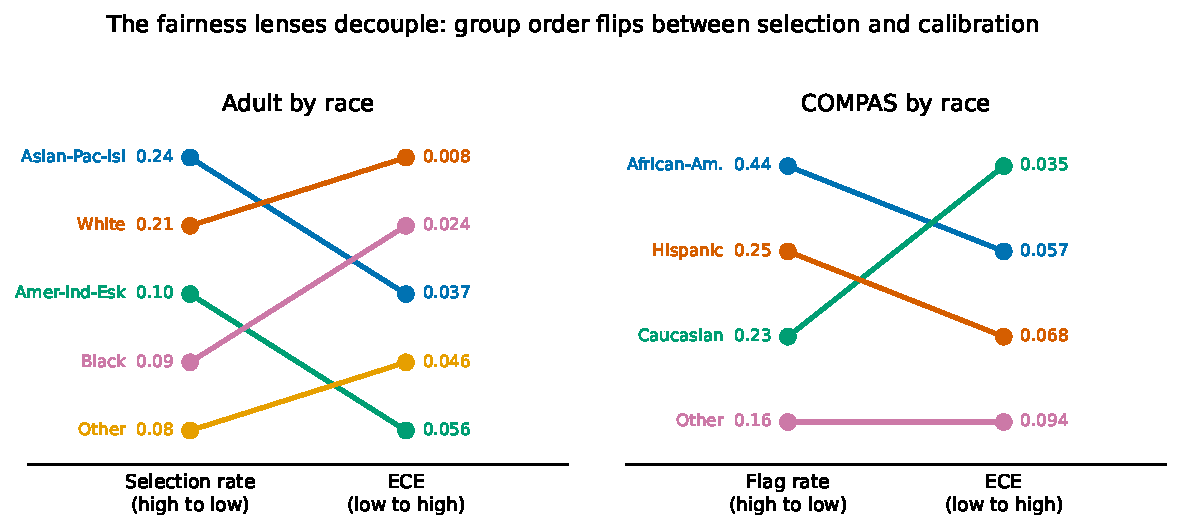
\includegraphics[width=0.72\linewidth]{figures/decoupling.pdf}
  \caption{Finding 1. Rank slope charts for Adult (left) and COMPAS (right) by race, uncompressed logistic model, means over 10 seeds. Each line joins a group's rank by selection/flag rate to its rank by per-group ECE. Crossing lines mean the two lenses order the groups differently.}
  \label{fig:decoupling}
\end{figure}

\textbf{Adult by race} (five groups). By selection rate Asian-Pacific-Islander ($0.240$) and White ($0.207$) rank highest and the smaller groups lowest; calibration reorders them. White is only second-most-selected yet by far the best calibrated (ECE $0.008 \pm 0.002$, three to seven times lower than every other group), while American-Indian-Eskimo is worst ($0.056 \pm 0.019$). The smaller groups carry higher, noisier calibration error that the selection view does not surface. \textbf{By sex} the disagreement inverts: a large selection gap (Male $0.253$ vs Female $0.079$) with negligible calibration difference (ECE $0.009$ vs $0.014$).

\textbf{COMPAS by race} (positive outcome = flagged high-risk, so higher is worse; groups with $n<10$ dropped). African-American defendants are flagged at roughly twice the rate of the next group ($0.441 \pm 0.015$ vs Hispanic $0.249 \pm 0.046$), the well-known point disparity. Yet the worst-calibrated group, Other (ECE $0.094 \pm 0.029$), is flagged \emph{least} ($0.164 \pm 0.033$), and the best calibrated is Caucasian ($0.035 \pm 0.016$). The reordering therefore holds on a second dataset whose favorable direction is inverted, so it is not an Adult-specific label-convention artifact.

\textbf{Why it matters on-device.} Sensitive labels are rarely available at inference time, so on-device audit triggers lean on confidence scores as a proxy \cite{kenfack2024}; if the lenses disagree about which group is worst served, a uniform confidence threshold can track the wrong disparity \cite{rosenblatt2024,kuzucu2024}. Reporting both is the cheap fix, and TinyAudit does so by construction.

\section{Result 2: one-shot compression hides unfairness; fine-tuning confines it}
\label{sec:finding2}

\begin{figure}[t]
  \centering
  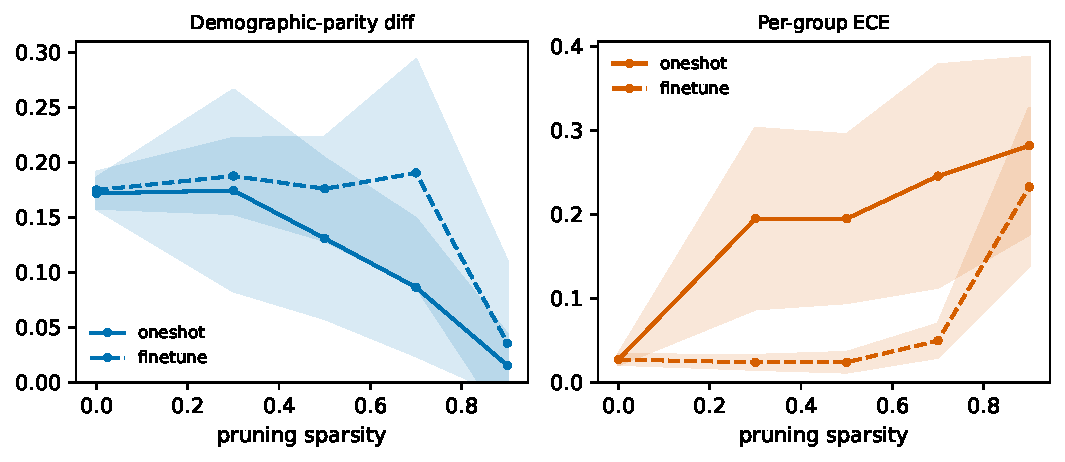
\includegraphics[width=\linewidth]{figures/compression_finetune.pdf}
  \caption{Finding 2. Adult MLP by sex under magnitude pruning, one-shot (solid) vs prune-then-fine-tune (dashed); bands are $\pm 1$ std over 10 seeds. One-shot pruning drives demographic parity down and per-group ECE up at every sparsity; fine-tuning holds both flat through 70\% and lets only a residual reappear at 90\%, where accuracy can no longer be recovered.}
  \label{fig:compression}
\end{figure}

We prune the Adult MLP to increasing sparsity and re-run the full audit at each level under two protocols that differ in exactly one step: one-shot magnitude pruning, and pruning followed by masked fine-tuning, in which the surviving weights are retrained while the pruned weights are held at zero --- the standard deployment practice (Figure~\ref{fig:compression}).

\textbf{One-shot pruning produces the divergence at every level.} By sex, demographic parity falls from $0.172 \pm 0.014$ to $0.015 \pm 0.028$ at 90\% while per-group ECE climbs from $0.027 \pm 0.006$ to $0.282 \pm 0.105$; by race, DP $0.152 \rightarrow 0.022$ and ECE $0.050 \rightarrow 0.314$. But the model degrades at every rung: accuracy falls to $0.50$ at 90\%, below the $0.76$ majority-class rate. It looks fairer on parity precisely as it stops predicting.

\textbf{Fine-tuning removes the divergence through 70\% sparsity.} Retraining the survivors keeps accuracy at $0.77$--$0.84$ through 70\% sparsity, and with it demographic parity stays put (sex $\approx 0.18$, race $\approx 0.16$) and per-group ECE stays low ($0.02$--$0.07$). Up to aggressive sparsity, the one-shot divergence is an artifact of skipping the fine-tuning step.

\textbf{A residual survives only at 90\%, where the model breaks anyway.} There fine-tuning cannot restore the model (accuracy $0.59 \pm 0.24$, still below the majority rate) and a weakened divergence returns (sex DP $0.036$, ECE $0.233$; race DP $0.036$, ECE $0.262$). Seed-paired against one-shot at 90\%, fine-tuning significantly lowers the calibration damage (ECE $\Delta = -0.05$, 95\% CI $[-0.08, -0.02]$) but does not significantly change the parity collapse ($\Delta = +0.02$, CI crosses zero). The COMPAS logistic model at 90\% one-shot pruning shows the same endpoint in the extreme: it predicts one class for everyone, giving DP $=0$ and DI $=1$, perfect parity by construction.

The upshot for auditors is protocol-independent: a parity-only audit cannot tell a healthy fine-tuned model from a collapsed one --- both can read DP $\approx 0$ --- so calibration has to be measured on the compressed artifact, whichever protocol shipped it.

\section{Result 3: the uncertainty lens is not the calibration lens}
\label{sec:finding3}

We call the audit uncertainty-aware, so it is fair to ask whether the uncertainty view adds anything the calibration view does not already give: per-group ECE also reads confidence, so is ``uncertainty-aware'' just ``calibration-aware'' renamed? We test it directly. From the same perturbation ensemble we take the pure uncertainty quantities it already produces (per-group predictive entropy, ensemble variance, and mutual information) and ask whether they single out a \emph{different} group than calibration does (Figure~\ref{fig:uncsig}, Appendix~\ref{app:uncsig}).

They do. Over 10 seeds the mean absolute Spearman correlation between the entropy ordering and the ECE ordering is $0.21$ across the three race cells (Adult logistic $-0.40$, Adult MLP $+0.18$, COMPAS logistic $-0.06$), so the two lenses do not rank the groups together. Entropy is not noise: on Adult it tracks the \emph{selection-rate} ordering (Spearman $\approx +0.75$), so it forms its own axis rather than restating calibration. On sex (two groups, so the contrast is a disparity gap rather than a correlation) the entropy gap between groups is large where the ECE gap is negligible (Adult $0.154$ vs $0.006$; Adult MLP $0.155$ vs $0.023$). We also report the one cell where the two agree (COMPAS by sex, where the ECE gap is the larger of the two). The uncertainty view therefore adds information that a calibration-only audit would miss. The one-shot Result~2 collapse also replicates on ACSIncome, a third and larger Census benchmark (Appendix~\ref{app:acsincome}).

\section{Feasibility: what the audit itself costs}
\label{sec:feasibility}

Audit tooling is normally not profiled at all: the model's footprint is reported and the auditor's is assumed free because it runs on a workstation. If the audit is to run where the model runs, that assumption has to be checked. We profile the full three-method audit with \texttt{tracemalloc} and report the pipeline's own peak RAM and wall-clock, not the audited model's (Table~\ref{tab:footprint}, Appendix~\ref{app:footprint}).

The working set is dominated by per-sample buffers: the feature matrix, the ensemble's stacked prediction arrays, and the explainer's perturbation batch. Two regimes appear across the Adult logistic sweep (Table~\ref{tab:footprint}): a fixed floor of about $0.6$\,MB that dominates at small batches ($610$\,KB at batch 64, $641$\,KB at batch 256, essentially flat) and a per-sample term of about $2.4$\,KB that dominates once the batch is large ($2.48$\,MB at 1024, $9.83$\,MB at 4096, a slope through a near-zero intercept). A single additive fit overstates the middle of the range by nearly a factor of two, so the honest summary is the larger of the two terms:
\begin{equation}
  \text{peak RAM} \approx \max\!\left(0.6\,\text{MB},\; 2.4\,\text{KB} \times \text{batch size}\right),
\end{equation}
the two crossing near a batch of 256. The structural claim is straightforward: an arbitrarily large test set streams through the audit in fixed-size batches at constant peak RAM, so audit cost is set by the batch size the engineer picks, not by how much test data exists. Against the standard toolkit the in-house metric path is not the bottleneck: TinyAudit's point-fairness stage returns the identical demographic-parity value as Fairlearn (its reference oracle) while using 8--11$\times$ less peak memory (e.g.\ 164 vs 1{,}352 KB at a 4096-row batch on Adult, 47 vs 514 KB on COMPAS).

The absolute constant needs more care. At a 256-row batch the audit peaks at 0.61 to 0.95 MB in under 0.1 s: not within the 32 to 512 KB parts at the low end of the TinyML range, but within reach of the high end, such as Cortex-M7 parts with roughly 1 MB of SRAM. The engineer controls only the per-sample term, not the 0.6 MB fixed cost, so driving that fixed cost below 512 KB is the concrete target this measurement identifies. Two caveats: the audited Adult MLP itself peaks at 6.0 MB, so it stands in for an MCU-class model rather than being one (the 62 KB COMPAS logistic model is the realistic case), and \texttt{tracemalloc} excludes the interpreter while counting Python overhead a compiled port would avoid. The scaling law is robust; the absolute constant is not.

\section{Limitations and conclusion}
\label{sec:limitations}

Features are standardized before fitting, so the numbers describe the scaled-input regime. The uncertainty ensemble is five lightly-jittered copies of the compressed model, not five retrains, so uncertainty magnitudes are relative. The prune-then-fine-tune arm covers the MLP; the logistic and ACSIncome compression results are reported under one-shot pruning only, and whether fine-tuning likewise confines their collapse is left to future work. int8 models' float weights are unreachable, so their uncertainty columns are blank; decision trees have no dense weights and sit out the compression grid. Footprint numbers are measured on x86, not on a microcontroller. The explainability stage yields no fairness result: the top-$k$ feature divergence between groups is non-monotone under pruning, within seed noise, and does not replicate on COMPAS, so we report that stage as instrument and cost, not evidence. Neither result we do report is theoretically novel \cite{kleinberg2017,chouldechova2017,hooker2020}; the contribution is measuring them on the model that ships, where those effects prove measurable, group-selective, and --- under one-shot pruning at any sparsity, and even after fine-tuning at aggressive sparsity --- actively misleading, at under a megabyte per streaming batch: a parity-only audit cannot separate a healthy compressed model from a collapsed one.

\begin{thebibliography}{19}

\bibitem{angwin2016}
J. Angwin, J. Larson, S. Mattu, and L. Kirchner.
\newblock Machine bias.
\newblock \emph{ProPublica}, 2016.

\bibitem{deng2022}
W. H. Deng et al.
\newblock Exploring how machine learning practitioners (try to) use fairness toolkits.
\newblock In \emph{Proc. ACM Conference on Fairness, Accountability, and Transparency (FAccT)}, 2022.

\bibitem{blakeney2021}
C. Blakeney, N. Huish, Y. Yan, and Z. Zong.
\newblock Simon says: Evaluating and mitigating bias in pruned neural networks with knowledge distillation.
\newblock arXiv:2106.07849, 2021.

\bibitem{chouldechova2017}
A. Chouldechova.
\newblock Fair prediction with disparate impact: A study of bias in recidivism prediction instruments.
\newblock \emph{Big Data}, 5(2):153--163, 2017.

\bibitem{ding2021}
F. Ding, M. Hardt, J. Miller, and L. Schmidt.
\newblock Retiring Adult: New datasets for fair machine learning.
\newblock In \emph{Advances in Neural Information Processing Systems (NeurIPS)}, 2021.

\bibitem{fabris2022}
A. Fabris, S. Messina, G. Silvello, and G. A. Susto.
\newblock Algorithmic fairness datasets: the story so far.
\newblock \emph{Data Mining and Knowledge Discovery}, 36(6):2074--2152, 2022.

\bibitem{ghanathe2025}
N. Ghanathe and S. Wilton.
\newblock QUTE: Quantifying uncertainty in TinyML models with early-exit-assisted ensembles for model-monitoring.
\newblock In \emph{Proc. International Conference on Machine Learning (ICML)}, PMLR vol. 267, 2025.

\bibitem{han2024}
X. Han, J. Chi, Y. Chen, Q. Wang, H. Zhao, N. Zou, and X. Hu.
\newblock FFB: A fair fairness benchmark for in-processing group fairness methods.
\newblock In \emph{Proc. International Conference on Learning Representations (ICLR)}, 2024.

\bibitem{hooker2020}
S. Hooker, N. Moorosi, G. Clark, S. Bengio, and E. Denton.
\newblock Characterising bias in compressed models.
\newblock arXiv:2010.03058, 2020.

\bibitem{kenfack2024}
P. J. Kenfack, S. E. Kahou, and U. A\"{i}vodji.
\newblock Fairness under demographic scarce regime.
\newblock \emph{Transactions on Machine Learning Research (TMLR)}, 2024.

\bibitem{kleinberg2017}
J. Kleinberg, S. Mullainathan, and M. Raghavan.
\newblock Inherent trade-offs in the fair determination of risk scores.
\newblock In \emph{Proc. Innovations in Theoretical Computer Science (ITCS)}, 2017.

\bibitem{kohavi1996}
R. Kohavi and B. Becker.
\newblock UCI Adult (Census Income) data set.
\newblock UCI Machine Learning Repository, 1996.

\bibitem{kuzucu2024}
S. Kuzucu, J. Cheong, H. Gunes, and S. Kalkan.
\newblock Uncertainty as a fairness measure.
\newblock \emph{Journal of Artificial Intelligence Research (JAIR)}, 2024.

\bibitem{lee2021}
M. S. A. Lee and J. Singh.
\newblock The landscape and gaps in open source fairness toolkits.
\newblock In \emph{Proc. CHI Conference on Human Factors in Computing Systems}, 2021.

\bibitem{nguyen2024}
T. Nguyen, D. Nguyen, and H. Cao.
\newblock XEdgeAI: A human-centered industrial inspection framework with data-centric explainable edge AI approach.
\newblock \emph{Information Fusion}, vol. 116, 2024.

\bibitem{pleiss2017}
G. Pleiss, M. Raghavan, F. Wu, J. Kleinberg, and K. Q. Weinberger.
\newblock On fairness and calibration.
\newblock In \emph{Advances in Neural Information Processing Systems (NeurIPS)}, 2017.

\bibitem{rosenblatt2024}
L. Rosenblatt and R. T. Witter.
\newblock FairlyUncertain: A comprehensive benchmark of uncertainty in algorithmic fairness.
\newblock arXiv:2410.02005, 2024.

\bibitem{salih2025}
A. Salih, I. B. Galazzo, P. Gkontra, et al.
\newblock A perspective on explainable artificial intelligence methods: SHAP and LIME.
\newblock \emph{Advanced Intelligent Systems}, 2025.

\bibitem{somvanshi2025}
S. Somvanshi, M. Islam, S. Chhetri, S. Chakraborty, et al.
\newblock From tiny machine learning to tiny deep learning: A survey.
\newblock \emph{ACM Computing Surveys}, 2025.

\end{thebibliography}

\appendix

\section{Uncertainty-vs-calibration rank charts}
\label{app:uncsig}

Figure~\ref{fig:uncsig} shows the per-cell rank slope charts underlying Result~3. The main-text numbers (mean $|\rho| = 0.21$ across the race cells; the per-cell Spearman values; the sex disparity contrast) are self-contained; this figure is the visual form of that finding.

\begin{figure}[h]
  \centering
  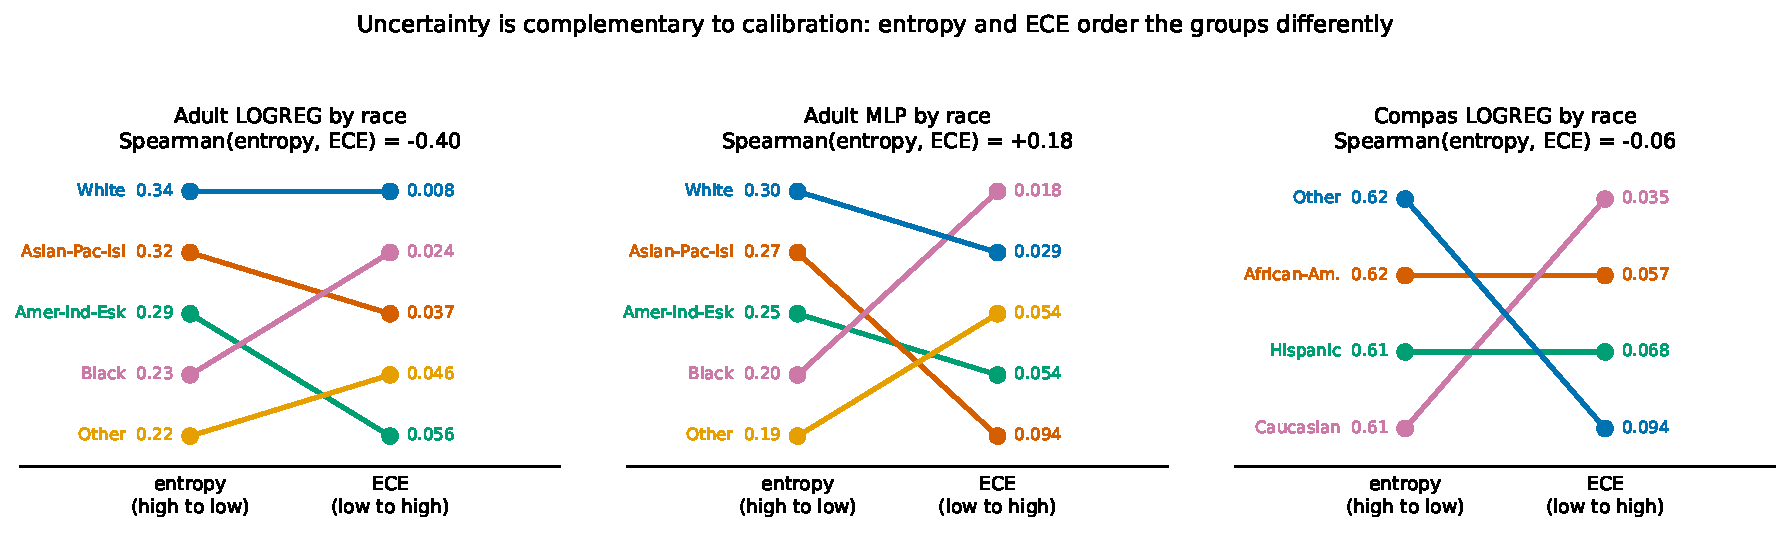
\includegraphics[width=\linewidth]{figures/uncertainty_vs_calibration.pdf}
  \caption{Rank slope charts by race for the three framing-critical cells, uncompressed, means over 10 seeds. Each line joins a group's rank by predictive entropy to its rank by per-group ECE; crossing lines mean the uncertainty and calibration lenses order the groups differently. Panel titles give the per-cell Spearman rank correlation.}
  \label{fig:uncsig}
\end{figure}

\section{ACSIncome replication of the compression collapse}
\label{app:acsincome}

Under one-shot pruning, the Result~2 effect is not specific to Adult and COMPAS. On ACSIncome (logistic, three seeds, test set subsampled to 8{,}000 rows for cost), pruning to 90\% sparsity drives the demographic-parity difference by sex from $0.034$ to $0.000$ while accuracy collapses from $0.781$ to $0.589$ and the positive-prediction rate falls to zero --- the ``fairest'' model in the sweep is again the most broken --- and per-group ECE disparity rises from $0.008$ to $0.112$. The same silent-collapse mechanism appears on a modern, larger Census benchmark.

\section{Audit pipeline footprint}
\label{app:footprint}

\begin{table}[h]
  \caption{Audit pipeline footprint (the pipeline itself, not the audited model), profiled with \texttt{tracemalloc} over 3 seeds. Peak RAM is governed by the streaming batch size, not the test-set size.}
  \label{tab:footprint}
  \centering
  \begin{tabular}{llrrr}
    \toprule
    Dataset & Model & Batch & Audit peak RAM (KB) & Audit wall-clock (s) \\
    \midrule
    Adult  & logreg & 64   & 610   & 0.03 \\
    Adult  & logreg & 256  & 641   & 0.06 \\
    Adult  & logreg & 1024 & 2{,}477 & 0.11 \\
    Adult  & logreg & 4096 & 9{,}826 & 1.10 \\
    Adult  & MLP    & 256  & 946   & 0.08 \\
    Adult  & MLP    & 4096 & 9{,}824 & 1.28 \\
    COMPAS & logreg & 256  & 609   & 0.01 \\
    COMPAS & MLP    & 1543 & 1{,}181 & 0.05 \\
    \bottomrule
  \end{tabular}
\end{table}

\end{document}
